\section*{Problem Statement}
The objective of this problem is to solve the classical harmonic oscillator equation numerically using LU decomposition. The oscillator follows the equation of motion:
\[
  m \frac{d^2x}{dt^2} + kx = 0,
\]
where $m$ is the mass and $k$ is the spring constant. The method discretizes the second-order ODE and formulates a system of linear equations that is solved using LU decomposition.

\begin{quote}
  \textbf{NOTE}: The code can be accessed using this link: \href{https://raw.githubusercontent.com/HavokSahil/computational-techniques-assignments/refs/heads/main/assignment2/a2.m}{MATLAB}, \href{https://raw.githubusercontent.com/HavokSahil/computational-techniques-assignments/refs/heads/main/assignment2/a2.jl}{Julia}.
\end{quote}

\section*{Methodology}
The equation of motion is discretized using the finite-difference approximation:
\[
  x_{n+1} = \frac{k \, \Delta t^2}{m} x_n - 2x_n + x_{n-1},
\]
where $\Delta t$ is the time step. This recurrence relation is transformed into a tridiagonal linear system:
\[
  AX = B,
\]
where $A$ is constructed from the discretized coefficients, and $B$ encodes initial conditions.

The solution proceeds as follows:
\begin{enumerate}
  \item Construct the coefficient matrix $A$ from the finite-difference scheme.
  \item Form the right-hand side vector $B$ using initial conditions $x_0$ and $x_1$.
  \item Apply LU decomposition to factorize $A = LU$. See \eqref{eq:computeu} and \eqref{eq:computel}
  \item Solve the system by:
\begin{enumerate}
  \item $LY = B \quad \text{(forward substitution)} \hfill \eqref{eq:forsubs}$
  \item $UX = Y \quad \text{(backward substitution)} \hfill \eqref{eq:backsubs}$
\end{enumerate}
  \item Reconstruct the full displacement vector $Z(t)$ including the initial values.
  \item Plot the solution $x(t)$ against $t$.
\end{enumerate}

\section*{Results}
For the chosen parameters:
\[
  m = 0.01, \quad k = 5.0, \quad \Delta t = 0.01, \quad t_{\max} = 2, \quad x(0) = 0, \quad v(0) = 0.5,
\]
the computed trajectory of the oscillator is shown in Figure~\ref{fig:a2}.

\begin{figure}[h!]
  \centering
  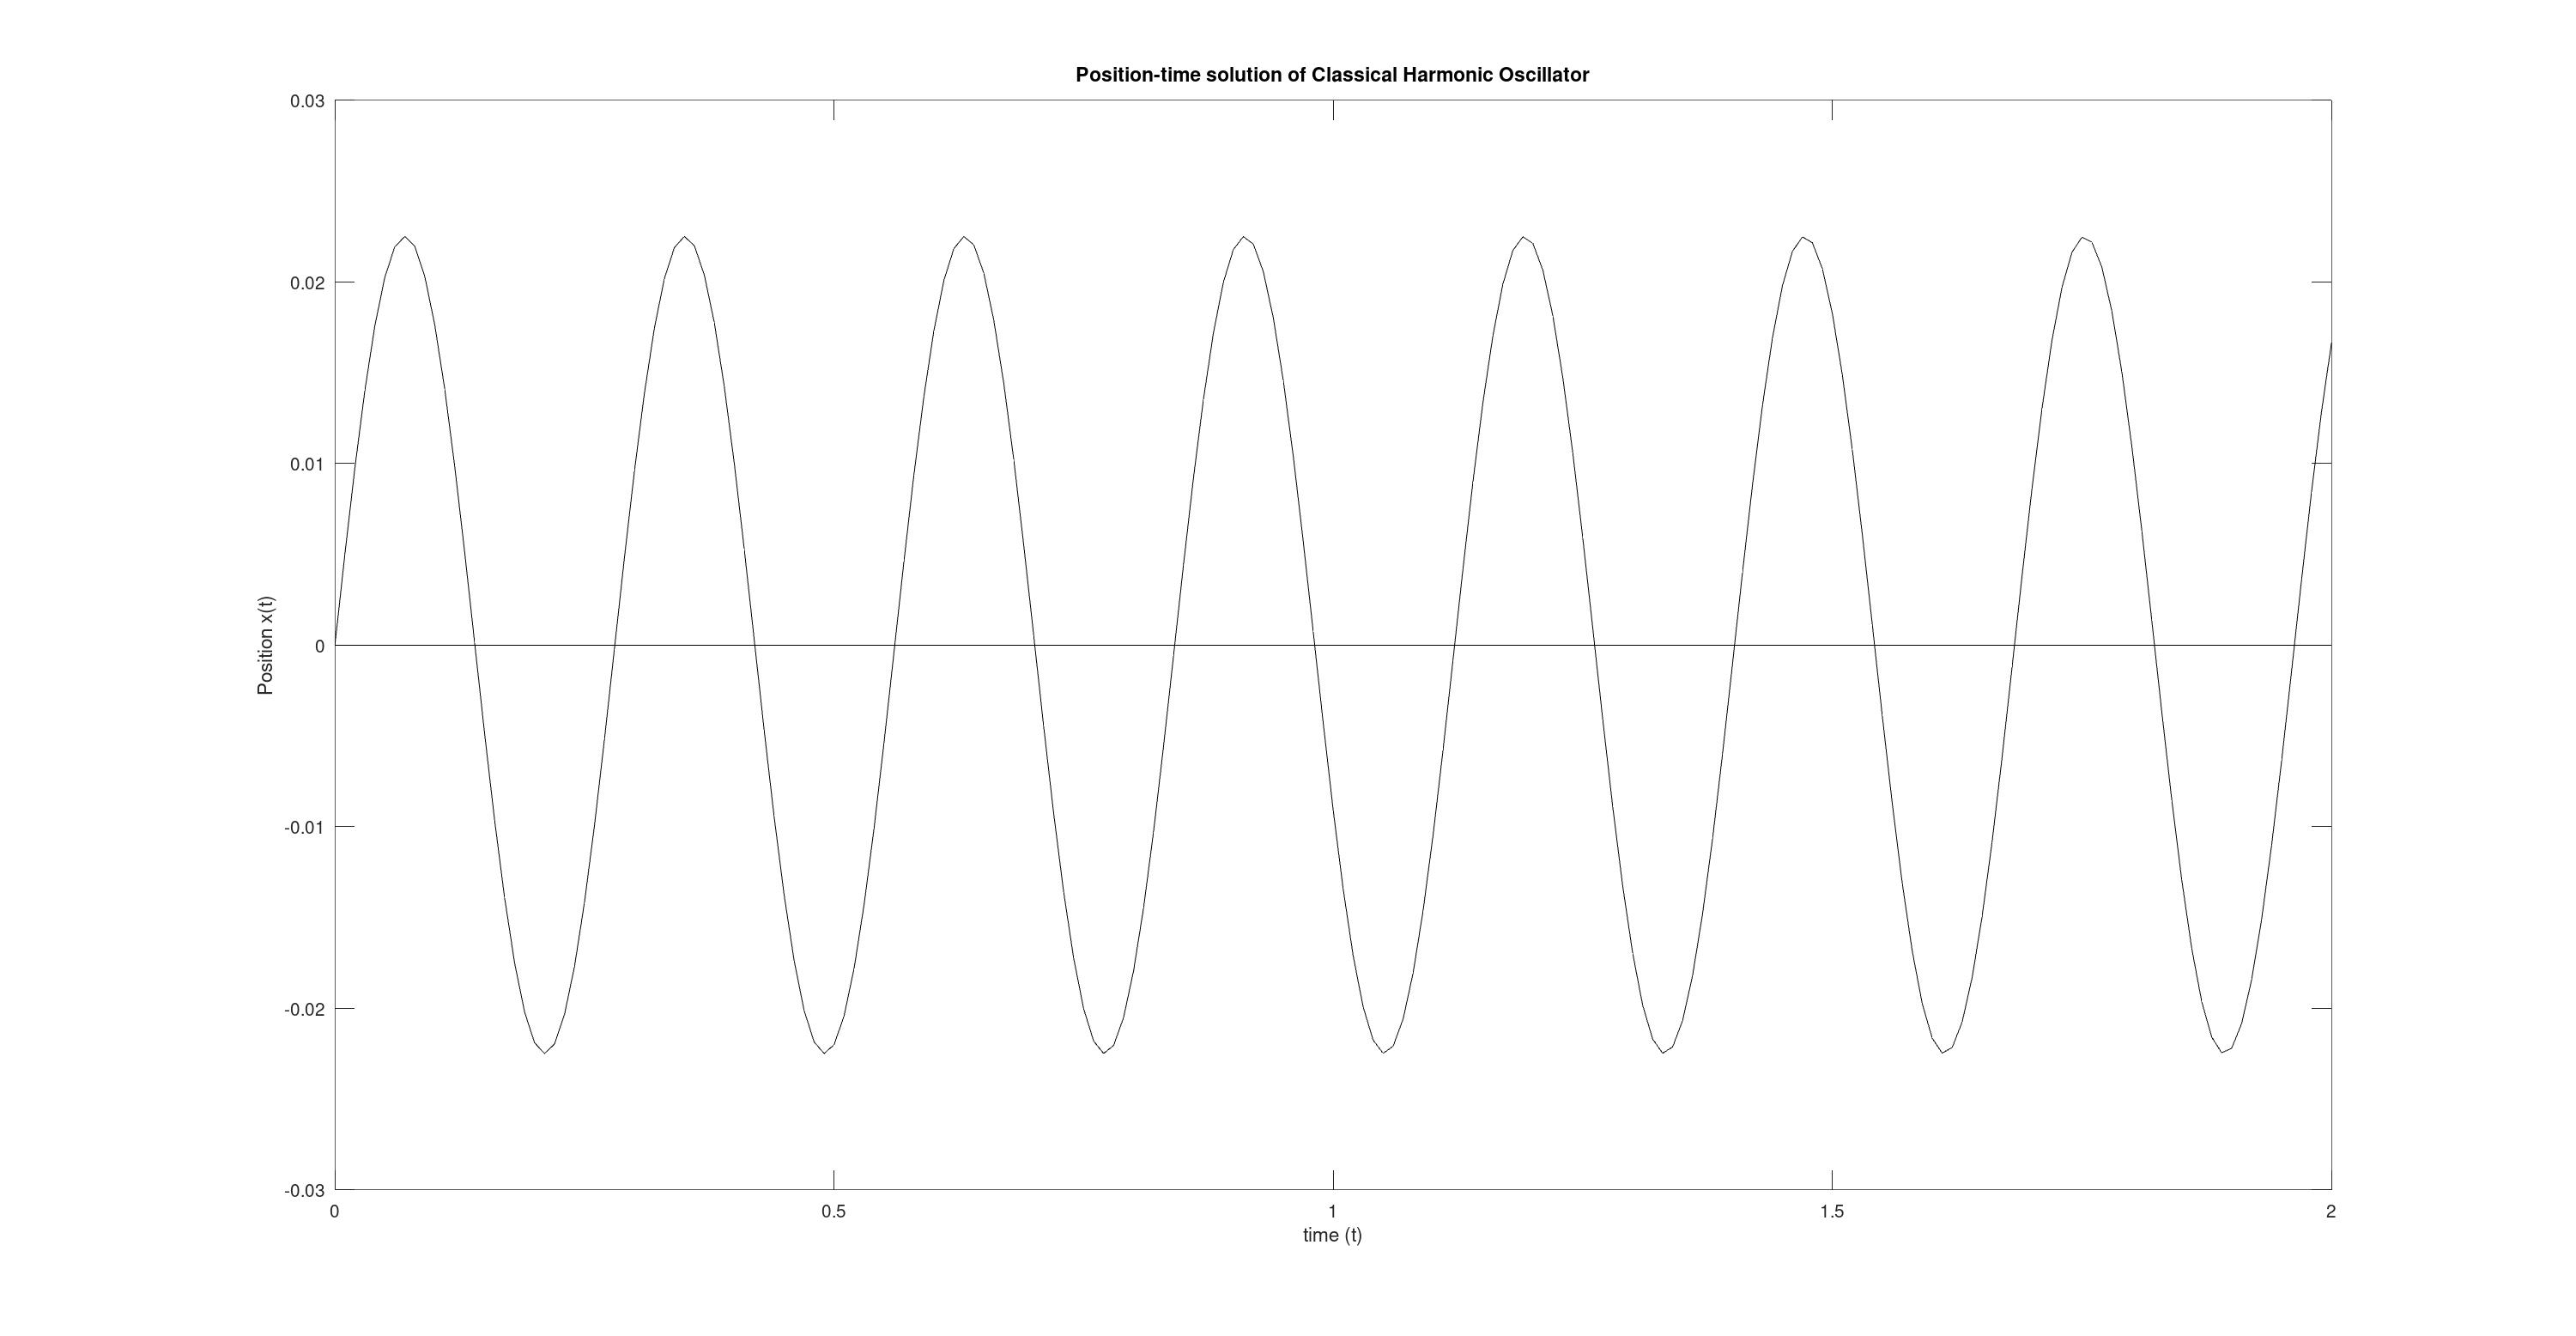
\includegraphics[width=1.0\textwidth]{a2.jpg}
  \caption{Numerical solution of the classical harmonic oscillator using LU decomposition.}
  \label{fig:a2}
\end{figure}

The plot shows a sinusoidal oscillation with the expected period $T = 2\pi \sqrt{m/k}$, consistent with the analytical solution of the harmonic oscillator.

\section*{Conclusion}
The LU decomposition method was successfully applied to solve the classical harmonic oscillator problem. By converting the discretized second-order ODE into a linear system, the problem reduces to triangular substitutions after decomposition. The numerical solution matches the expected sinusoidal oscillation, demonstrating the correctness of the method. This approach highlights the usefulness of LU decomposition in solving time-stepping problems arising in physics and engineering.
